\documentclass[border=2mm,tikz]{standalone}

\usepackage{tikz}
\usetikzlibrary{arrows.meta}
% \usetikzlibrary{decorations.pathmorphing} 
% \usetikzlibrary{background}
\usetikzlibrary{positioning}
% \usetikzlibrary{fit}
% \usetikzlibrary{petri}

\begin{document}
    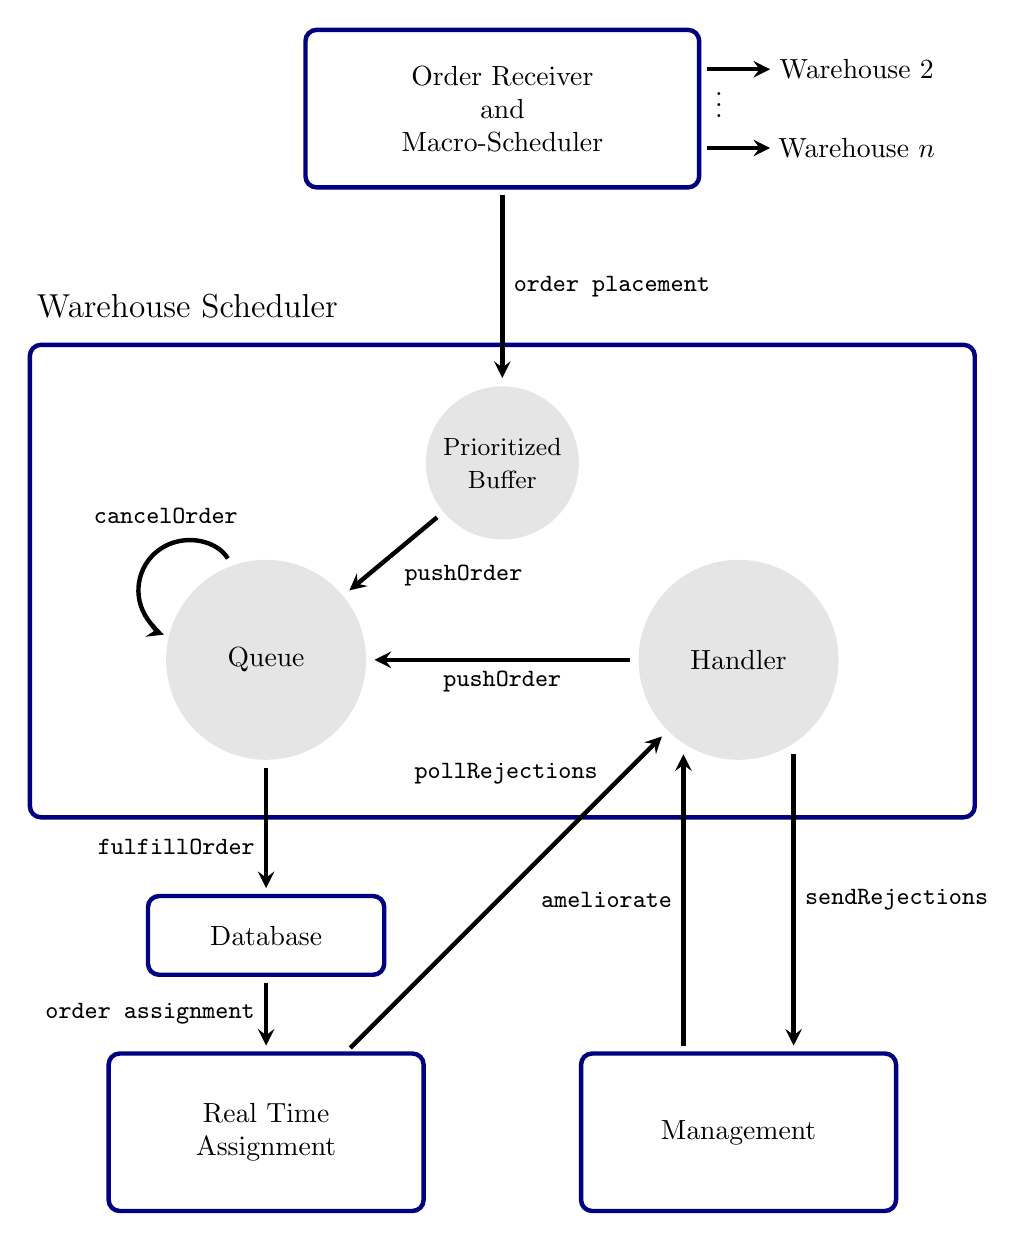
\begin{tikzpicture}[
        arrow/.style={-stealth,ultra thick,shorten >= 1mm, shorten <= 1mm},
        frame/.style={rounded corners,draw=blue!50!black,ultra thick},
        inside/.style={circle,fill=white!90!black,minimum size=1in},
        inside small/.style={minimum size=0.75in},
    ]
        % macro
        \draw[frame] (-2.5,5) rectangle (2.5,7);
        \node[align=center] at (0,6)
            {Order Receiver\\and\\Macro-Scheduler};

        \draw[arrow] (2.5,6.5) -- (3.5,6.5);
        \node at (2.75,6.15) {$\vdots$};
        \draw[arrow] (2.5,5.5) -- (3.5,5.5);

        \node[align=left] at (4.5,6.5) {Warehouse 2};
        \node[align=left] at (4.5,5.5) {Warehouse $n$};

        % warehouse
        \draw[frame] (-6,-3) rectangle (6,3);
        \node at (-4,3.5) {\large Warehouse Scheduler};

        \node (buffer)  at (0,1.5) [inside,inside small,align=center]
            {\small Prioritized\\\small Buffer};
        \node (queue)   at (-3,-1) [inside]              {Queue};
        \node (handler) at (3,-1)  [inside]              {Handler};

        \draw[arrow] (buffer) -- (queue) node[midway,below right]
            {\small \verb|pushOrder|};

        \draw[arrow] (queue.110) arc (30:250:0.25in)
            node[midway,above,xshift=2mm,yshift=3mm]
            {\small \verb|cancelOrder|};

        \draw[arrow] (handler) -- (queue) node[midway,below]
            {\small \verb|pushOrder|};
        
        \draw[arrow] (0,5) -- (buffer) node[midway,right]
            {\small \verb|order placement|};

        % buffer
        \draw[frame] (-4.5,-5) rectangle (-1.5,-4);
        \node[align=center] at (-3,-4.5) {Database};

        \draw[arrow] (queue) -- (-3,-4) node[midway,below left]
            {\small \verb|fulfillOrder|};

        % rts
        \draw[frame] (-5,-8) rectangle (-1,-6);
        \node[align=center] at (-3,-7) {Real Time\\Assignment};

        \draw[arrow] (-3,-5) -- (-3,-6) node[midway,left]
            {\small \verb|order assignment|};

        \draw[arrow] (-2,-6) -- (handler)
            node[midway,yshift=1.5cm]
            {\small \verb|pollRejections|};

        % manager
        \draw[frame] (5,-8) rectangle (1,-6);
        \node[align=center] at (3,-7) {Management};

        \draw[arrow] (2.3,-6) -- (2.3,-2.1) node[midway,left]
            {\small \verb|ameliorate|};
        \draw[arrow] (3.7,-2.1) -- (3.7,-6) node[midway,right]
            {\small \verb|sendRejections|};
    \end{tikzpicture}
\end{document}